\documentclass{article}
\usepackage{epsfig}
\usepackage{psfrag}

\bibliographystyle{plain}

%&t&{\tt #}&
%&v&\verb|#|&
\newcounter{lemma1}
\newtheorem{theorem}{Theorem}
\newtheorem{conjecture}[theorem]{Conjecture}
\newtheorem{corollary}[theorem]{Corollary}
\newtheorem{proposition}[theorem]{Proposition}
\newtheorem{lemma}[lemma1]{Lemma}

% Texts on the EPS figures.
%
\psfrag{zs}{$s$}
\psfrag{zt}{$t$}
\psfrag{zt0}{$t_0$}
\psfrag{zs-Xpaths}{$s$-$X$ paths}
\psfrag{zGs+}{$G_s^+$}
\psfrag{zX}{$X$}
\psfrag{zX1*}{$X_1^*$}
\psfrag{zX1a}{$X_1^a$}
\psfrag{zX1n}{$X_1^n$}
\psfrag{z(a)}{(a)}
\psfrag{z(b)}{(b)}
\psfrag{z(c)}{(c)}
\psfrag{zNGs+-X1a(X1n)}{$N_{G_s^+ - X_1^a}(X_1^n)$}
\psfrag{zGs+-X1a}{$G_s^+ - X_1^a$}
\psfrag{zG1-X1a}{$G_1 - X_1^a$}
\psfrag{zM1*}{$M_1^*$}
\psfrag{zVM1*}{$V_{M_1^*}$}
\psfrag{zG1-X1a/M1*}{$(G_1 - X_1^a)/M_1^*$}
\psfrag{zx'inX1*}{$x' \in X_1^*$}
\psfrag{zxinXr*}{$x \in X_r^*$}
\psfrag{zxinGr}{$x \in G_r$}
\psfrag{zXr*}{$X_r^*$}
\psfrag{zX}{$X$}
\psfrag{zY}{$Y$}
\psfrag{zX0}{$X_0$}
\psfrag{zY0}{$Y_0$}
\psfrag{zM0}{$M_0$}
\psfrag{zGb}{$G_\beta$}
\psfrag{zA0}{$A_0$}
\psfrag{zB0}{$B_0$}
\psfrag{zC0}{$C_0$}
\psfrag{zD0}{$D_0$}
\psfrag{zF0}{$F_0$}
\psfrag{zI0}{$I_0$}
\psfrag{zS0}{$S_0$}
\psfrag{zM}{$M$}
\psfrag{zEK0}{$E_{K_0}$}
\psfrag{zEK'0}{$E_{K'_0}$}
\psfrag{zJ-0}{$J_-^0$}
\psfrag{zL0}{$L^0$}
\psfrag{zQ0}{$Q_0$}
\psfrag{zQ'0}{$Q'_0$}
\psfrag{zJQ0}{$J_Q^0$}
\psfrag{zJR0}{$J_Q^0$}
\psfrag{zu0}{$u_0$}
\psfrag{zw}{$w$}
\psfrag{zR0}{$R_0$}
\psfrag{zA1}{$A_1$}
\psfrag{zB1}{$B_1$}
\psfrag{zC1}{$C_1$}
\psfrag{zD1}{$D_1$}
\psfrag{zF1}{$F_1$}
\psfrag{zI1}{$I_1$}
\psfrag{zS1}{$S_1$}
\psfrag{zEK1}{$E_{K_1}$}
\psfrag{zEK'1}{$E_{K'_1}$}
\psfrag{zX1}{$X_1$}
\psfrag{zY1}{$Y_1$}
\psfrag{zt1}{$t_1$}
\psfrag{zL1}{$L^1$}
\psfrag{zR1}{$R_1$}
\psfrag{zu1}{$u_1$}
\psfrag{zJR1}{$J_R^1$}
\psfrag{zLR1}{$L_R^1$}
\psfrag{zSn}{$S_n$}
\psfrag{zLR0-t0}{$L_R^0-t_0$}
\psfrag{zLR1-t1}{$L_R^1-t_1$}
\psfrag{zLRn-tn}{$L_R^n-t_n$}
\psfrag{zW}{$W$}
\psfrag{zNG(s)}{$N_G(s)$}
\psfrag{zv1}{$v_1$}
\psfrag{zG'}{$G'$}
\psfrag{zG'-v1}{$G'-v_1$}
\psfrag{zv2}{$v_2$}
\psfrag{zvl-k}{$v_{l-k}$}
\psfrag{zu2}{$u_2$}
\psfrag{zul-k}{$u_{l-k}$}
\psfrag{zS2}{$S_2$}
\psfrag{zSl-k}{$S_{l-k}$}
\psfrag{zvl}{$v_l$}
\psfrag{zv3}{$v_3$}
\psfrag{zvk}{$v_k$}
\psfrag{zvk+1}{$v_{k+1}$}
\psfrag{zuk-1}{$u_{k-1}$}
\psfrag{zuk}{$u_k$}
\psfrag{zleft}{left}
\psfrag{zright}{right}
\psfrag{zMa}{$M_a$}
\psfrag{zP}{$P$}

\psfrag{zGs}{$G_s$}
\psfrag{zGt}{$G_t$}

\psfrag{zs1}{$s_1$}
\psfrag{zsk-1}{$s_{k-1}$}
\psfrag{zsk}{$s_{k}$}
\psfrag{zt}{$t$}
\psfrag{za1}{$a_1$}
\psfrag{za2}{$a_2$}
\psfrag{zab-1}{$a_{\beta-1}$}
\psfrag{zab}{$a_{\beta}$}
\psfrag{zab+1}{$a_{\beta+1}$}
\psfrag{zam}{$a_m$}
\psfrag{za'}{$a'$}
\psfrag{zw1}{$w_1$}
\psfrag{zw2}{$w_2$}
\psfrag{zw3}{$w_3$}
\psfrag{zwb-1}{$w_{\beta-1}$}
\psfrag{zwb}{$w_{\beta}$}
\psfrag{zwb+1}{$w_{\beta+1}$}
\psfrag{zwb+2}{$w_{\beta+2}$}
\psfrag{zwk}{$w_k$}
\psfrag{zwbk}{$w_{\beta+k}$}
\psfrag{zwkpG}{$w_{\kappa(G)}$}
\psfrag{Wst}{$W(s, t)$}
\psfrag{D0}{$D_0=s$}
\psfrag{D1}{$D_1$}
\psfrag{D2}{$D_2$}
\psfrag{D3}{$D_3$}
\psfrag{Dk-1}{$D_{k-1}$}
\psfrag{Dk}{$D_k$}
\psfrag{NGS}{$N_G(s)$}
\psfrag{NG1S}{$N_{G'}(s_1)$}
\psfrag{NGk-1S}{$N_{G^{(k-1)}}(s_{k-1})$}
\psfrag{NGkS}{$N_{G^{(k)}}(s_{k})$}
\psfrag{zNGkS}{$N_{G^{(k)}}(s_{k})$}
\psfrag{zu11}{$u_{1,1}$}
\psfrag{zu12}{$u_{1,2}$}
\psfrag{zu13}{$u_{1,3}$}
\psfrag{zu1k}{$u_{1,\kappa(G)}$}
\psfrag{zu21}{$u_{2,1}$}
\psfrag{zu22}{$u_{2,2}$}
\psfrag{zu23}{$u_{2,3}$}
\psfrag{zu2k}{$u_{2,\kappa(G)}$}
\psfrag{zu31}{$u_{3,1}$}
\psfrag{zu32}{$u_{3,2}$}
\psfrag{zu33}{$u_{3,3}$}
\psfrag{zu3k}{$u_{3,\kappa(G)}$}
\psfrag{zum-21}{$u_{m-2,1}$}
\psfrag{zum-22}{$u_{m-2,2}$}
\psfrag{zum-23}{$u_{m-2,3}$}
\psfrag{zum-2k}{$u_{m-2,\kappa(G)}$}
\psfrag{zum-11}{$u_{m-1,1}$}
\psfrag{zum-12}{$u_{m-1,2}$}
\psfrag{zum-13}{$u_{m-1,3}$}
\psfrag{zum-1k}{$u_{m-1,\kappa(G)}$}
\psfrag{zum1}{$u_{m,1}$}
\psfrag{zum2}{$u_{m,2}$}
\psfrag{zum3}{$u_{m,3}$}
\psfrag{zumk}{$u_{m,\kappa(G)}$}
\psfrag{zU1}{$U_1$}
\psfrag{zU2}{$U_2$}
\psfrag{zU3}{$U_3$}
\psfrag{zUm-2}{$U_{m-2}$}
\psfrag{zUm-1}{$U_{m-1}$}
\psfrag{zUm}{$U_{m}$}

\title{A Proof of Vertex-disjoint Menger's Theorem by Bipartite Matching and Contraction}
\author{SHOICHIRO YAMANISHI}



\begin{document}

\maketitle

\begin{abstract}
A proof of vertex-disjoint Menger's theorem between two distinctive vertices $s$ and $t$ in $G$ is proposed.
Starting from a minimum separator $X$ and the component $G_t$ of $G - X$ to which $t$ belongs, $|X|$ vertex-disjoint
$s$-$X$ paths are found in $G - V(G_t)$ by recursively applying contraction to bipartite matchings of $X$.
Similarly, $|X|$ vertex-disjoint $X$-$t$ paths are found. Concatenating two paths at each vertex in $X$ yields
$|X|$ vertex-disjoint $s$-$t$ paths. The contraction of the bipartite matchings must not decrease the connectivity.
Existence of such bipartite matchings are proven by induction on $|X|$. 
\end{abstract}



\section{Introduction}
Menger's theorem is one of the early fundamental discoveries in graph theory.
Since the original theorem was proposed by Menger \cite{menger1}, some variants have been proposed,
which are roughly divided into
vertex-disjoint ones, e.g. Whitney \cite{whitney1},  and edge-disjoint one by Ford and Fulkerson \cite{fordfulkerson1}.
For the vertex-disjoint theorems, several proofs have been proposed
by Dirac \cite{dirac1}; B\"{o}hme, G\"{o}ring, and Harant \cite{bohmegoringharant1};
Pym \cite{pym1}; and Gr\"{u}nwald (later Gallai) \cite{grunwald1}.
Also, the edge-disjoint theorem is proven by the min-cut/max-flow theorem \cite{fordfulkerson1}.
Of all the variants, we prove the following vertex disjoint theorem.
\begin{theorem}\label{theorem1}
{\bf (Menger's Theorem)}\\Given a graph $G=(V,\,E)$, let $s$ and $t$ be two
distinct non-adjacent vertices in $G$. The size of the minimum $s$-$t$ separators
is equal to the maximum number of internally vertex-disjoint $s$-$t$ paths.
\end{theorem}
In this article, we call the minimum number of separating vertices between $s$ and $t$ {\it $s$-$t$ connectivity} of $G$
and denote it by $\kappa_G(s, t)$ hereinafter.

The purpose of this article is to propose a new proof by recursively applying contraction of
a maximum bipartite matching of a minimum $s$-$t$ separator in a graph.
We also briefly discuss the possibility of finding algorithms for determining $s$-$t$ connectivity
and maximum number of vertex-disjoint $s$-$t$ paths.

It is easy to see the maximum number of disjoint $s$-$t$ paths does not exceed $\kappa_G(s, t)$.
We prove that we can actually construct $\kappa_G(s, t)$ disjoint $s$-$t$ paths in $G$.
It is also trivial to prove the case for $\kappa_G(s, t)=0$, so the following discussion assumes
$\kappa_G(s, t)>0$.

\section{Proof}
%Put all the notational conventions here.
We follow the notational conventions in Diestel's \cite{diestel1}.
We treat a matching $M$ as a set of edges in a graph $G$.
We denote the graph obtained from $G$ by contracting all the edges in $M$ by $G/M$,
and the set of vertices in $G/M$ into which the edges in $M$ are contracted by $V_M$.

Let $k:=\kappa_G(s, t)$.
Let $X$ be a minimum $s$-$t$ separator ($X\cap\{s, t\}=\emptyset$).
Let $G_s$, $G_t$ be the two components of $G - X$ to which $s$ and $t$ belong respectively.
Let $G_s^+$, $G_t^+$ be $G[V(G_s)\cup X]$, $G[V(G_t)\cup X]$ respectively.
We prove $G_s^+$ has $k$ vertex-disjoint $s$-$X$ paths.
Similarly,  $G_t^+$ has $k$ vertex-disjoint $X$-$t$ paths by symmetry.
Concatenating the two paths at each vertex in $X$ from each of $s$-$X$ paths and $X$-$t$ paths in $G$
yields $k$ vertex-disjoint $s$-$t$ paths (Fig. \ref{label_fig1}).

\begin{figure}\begin{center}
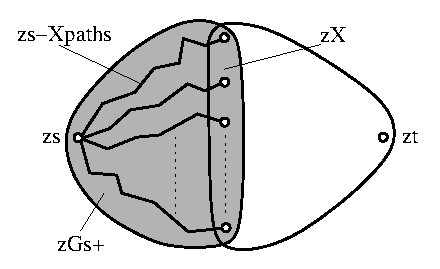
\epsfig{file=fig1.eps, width = 5cm}
\caption[Fig1]{$X$, $G_s^+$, and $s$-$X$ paths.}
\label{label_fig1}
\end{center}\end{figure}

The rest of the proof is for finding $k$ $s$-$X$ paths in $G_s^+$.
Our strategy is as follows. Let $G_1 := G$ and $X_1^* := X$.
Split $X_1^*$ into two subsets $X_1^a$ and $X_1^n$ such that
$X_1^a = \left\{ x\in X_1^* | \left\{s, x\right\}\in E(G_s^+)\right\}$ and
$X_1^n = \left\{ x\in X_1^* | \left\{s, x\right\}\not\in E(G_s^+)\right\}$ (Fig. \ref{label_fig2}(a)).
We have already found $|X_1^a|$ vertex-disjoint $s$-$X_1^*$ paths between $s$ and $X_1^a$ in $G_s^+$, each of which
is merely an edge.
\begin{figure}\begin{center}
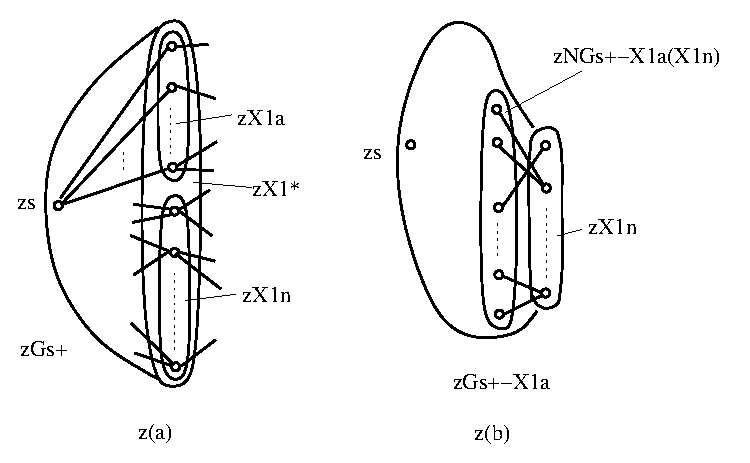
\epsfig{file=fig2.eps, height = 4cm}
\caption[Fig2]{$X_1^a$, $X_1^n$, and $G_s^+ - X_a$.}
\label{label_fig2}
\end{center}\end{figure}
Please observe that $X_1^n$ is a minimum separator of $G_1 - X_1^a$ (Fig. \ref{label_fig2}(b)).
It is easy to see $X_1^n$ is a separator of $G_1 - X_1^a$.
Suppose it were not minimum. Let $X'$ be a minimum separator of $G_1 - X_1^a$ such that $|X'| < |X_1^n|$.
Then $X' \cup X_1^a$ would give a minimum separator of $G_1$, which contradicts the minimality of $X_1^*$.

We prove there is a bipartite matching $M_1^*$ of $X_1^n$ to $N_{G_s^+ - X_1^a}(X_1^n)$ such that
$|M_1^*| = |X_1^n|$, and contracting all the edges in $M_1^*$ does not decrease the $s$-$t$ connectivity of $(G_1 - X_1^a)/M_1^*$,
i.e. $\kappa_{G_1 - X_1^a}(s, t) \le \kappa_{(G_1 - X_1^a)/M_1^*}(s, t)$ (Fig. \ref{label_fig3}(a)).
We eventually obtain the equality here since $V_{M_1^*} \cup X_1^a$
form an $s$-$t$ separator in $G_1/M_1^*$, which indicates they are again a minimum separator $X_2^*$ in $G_1/M_1^*$ and
$\kappa_{G_1}(s, t) = \kappa_{G_1/M_1^*}(s, t)$ (Fig. \ref{label_fig3}(b)). Let $G_2 = G_1/M_1^*$.
\begin{figure}\begin{center}
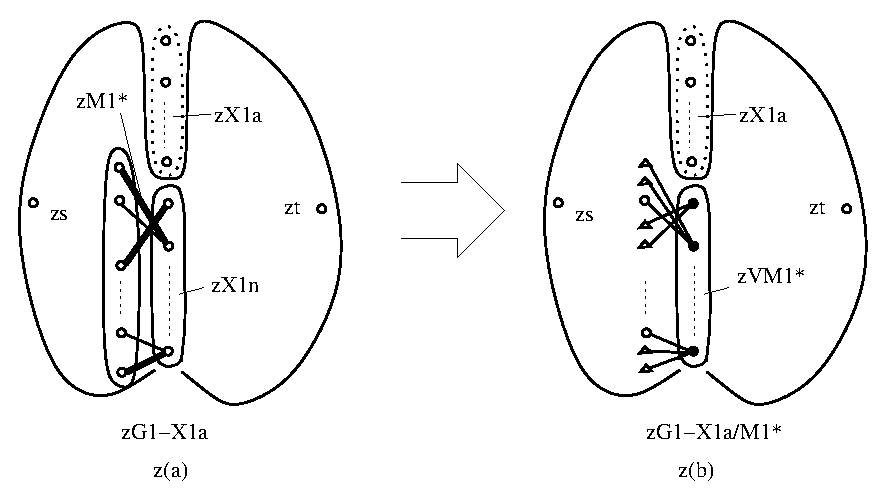
\epsfig{file=fig3.eps, height = 6cm}
\caption[Fig3]{$G_1 - X_1^a$, and $(G_1 - X_1^a)/M_1^*$.}
\label{label_fig3}
\end{center}\end{figure}

We can recursively apply this process of finding a matching and contracting all the edges in it
$r$ times until all the vertices in the minimum $s$-$t$ separator $X_r^*$ in $G_r$
 are adjacent to $s$ (Fig. \ref{label_fig4} (a)).
 This process is guaranteed to terminate as $G$ is finite,
and at each iteration at least one edge is contracted.
 If we ``unfold'' the edge $\{s, x\}$ and the vertex $x$ in $X_r^*$, to which some incident
edges have been contracted, we obtain  $|X|$ trees in $G_s^+$, which are mutually vertex-disjoint except at $s$.
In each tree we can find a unique $s$-$x'$ path for each $x'\in X_1^*$.
Those paths form a set of $k$ vertex-disjoint $s$-$X$ paths (Fig. \ref{label_fig4} (b)).

\begin{figure}\begin{center}
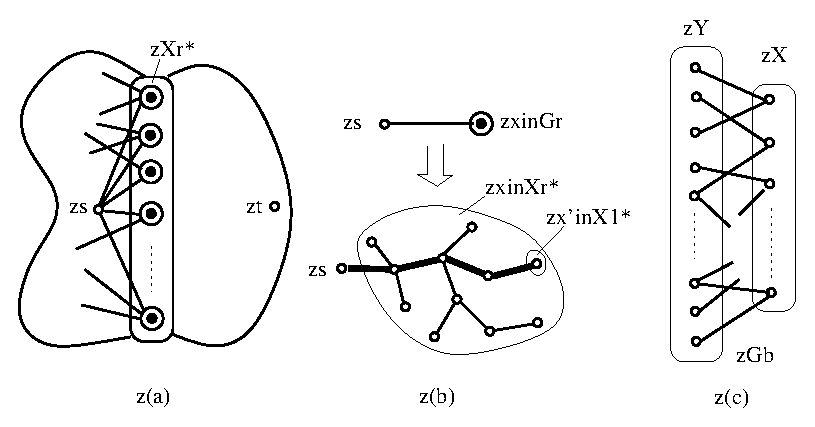
\epsfig{file=fig4.eps, width =10cm}
\caption[Fig4]{$G_r, X_r^*, and G_\beta$.}
\label{label_fig4}
\end{center}\end{figure}

The rest of the proof is dedicated to prove existence of a bipartite matching $M$
of $X_1^n$ to $N_{G_s^+ - X_1^a}(X_1^n)$ such that
contraction of all the edges in $M$ does not decrease the $s$-$t$ connectivity of in $G - X_1^a$.
In the following discussion, we assume $X_1^a = \emptyset$, i.e. $X = X_1^n$.
If  $X_1^a \ne \emptyset$, consider the graph $G - {X_1^a}$ instead of $G$ for its connectivity
$|X_1^n|$. We later add the edges (disjoint paths) in $X_1^a$, after we find vertex-disjoint
$s$-$X_1^n$ paths.


First we prove existence of a bipartite matching of $X$.
Let $Y := N_{G_s^+}(X)$. Since we assume $X_1^a$ is empty, $s$ is not in $Y$.
Consider the bipartite graph $G_\beta$ with the bipartition $\{X, Y\}$ (Fig. \ref{label_fig4} (c)).
Formally $G_\beta = G[X\cup Y] - \left(E\left(G[X]\right)\cup E\left(G[Y]\right)\right)$.
We can easily check that $G_\beta$ contains a bipartite matching of $X$.
Indeed, for all $S\subseteq X$, $d_{G_\beta}(S)\ge|S|$.
Suppose $\exists S \subseteq X$ such that $d_{G_\beta}(S) < |S|$, then
we can replace $S$ with $N_{G_\beta}(S)$ in $X$, which would be an $s$-$t$ separator in $G$
whose cardinality is less than $|X|$, which contradicts the minimality of $X$.
By the marriage theorem by Hall \cite{hall1}, $G_\beta$ contains a bipartite matching of $X$.

Next we prove existence of a bipartite matching $M$ of $X$ which does not reduce the $s$-$t$ connectivity
when contraction of $M$ is applied to $G$.
We prove this by induction on $\kappa_G(s, t)$, or on $|X|$.
If $|X| = 1$, it is trivial to prove contraction of any bipartite matching $M$ does not reduce
the $s$-$t$ connectivity. So the induction starts.

Let $X_0 := X$, $Y_0 := Y$, and $M_0$ be any bipartite matching of $X_0$ in $N_{G_\beta}$ (Fig. \ref{label_fig5}(a)).
 If it preserves the $s$-$t$ connectivity in $G/M_0$, we are done.
So we assume $\kappa_{G/M_0}(s, t) < \kappa_{G}(s, t)$.
$G/{M_0}$ has an $s$-$t$ separator $W_0$ in $G_s^+$ such that
$|W_0| < |X_0|$. $W_0$ contains at least one vertex in $V_{M_0}$,
otherwise $W_0$ would also be an $s$-$t$ separator in $G$ whose cardinality is less than $|X|$, a contradiction.
So $W_0\cap V_{M_0}\ne \emptyset$. Let $K_0 = W_0\cap V_{M_0}$ and $S_0 = W_0 \backslash K_0$.

Here we categorize the edges and vertices in $G$ for the following discussion (Fig. \ref{label_fig5}(b)).
\begin{itemize}
\item Let $E_{K_0}$ be the set of edges in $G$ which corresponds to $K_0$ in $G/M_0$.
\item Let $E_{K'_0}$ be $M_0\backslash E_{K_0}$.
\item Let $A_0$ and $C_0$ be the sets of vertices in $X_0$ and $Y_0$ respectively,
which are incident to the edges in $E_{K_0}$.
\item Let $B_0$ and $D_0$ be the sets of vertices in $X_0$ and $Y_0$ respectively, 
which are incident to the edges in $E_{K'_0}$.
\item Let $F_0$ be the set of vertices in $Y_0\backslash (C_0\cup D_0)$ which are not incident to any vertices in $B_0$.
\item Let $I_0$ be the set of vertices in $Y_0\backslash (C_0\cup D_0)$ which are incident to any vertices in $B_0$.
\end{itemize}
Please observe that $A_0 \cup C_0 \cup S_0$ separates $s$ from $t$ in $G$,
since $K_0 \cup S_0$ separates $s$ from $t$ in $G/M_0$.
Please also note that $S_0$ can be $\emptyset$, but neither $B_0$ nor $D_0$ can be empty.

\begin{figure}\begin{center}
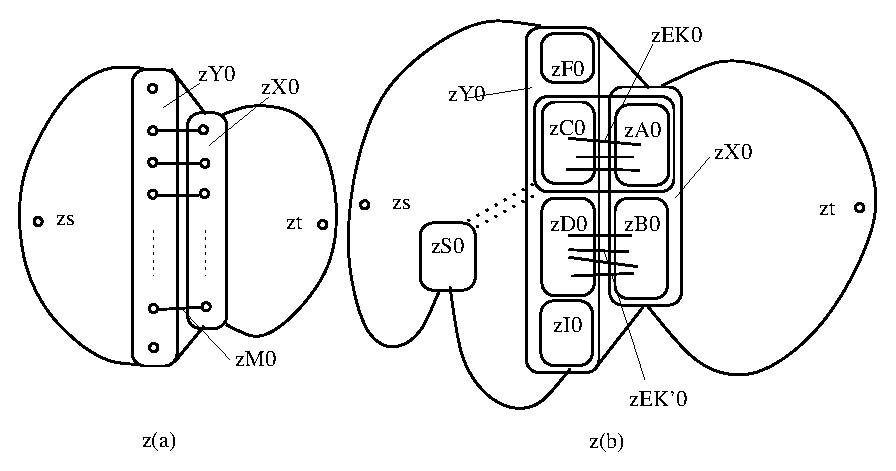
\epsfig{file=fig5.eps, height=6cm}
\caption[Fig5]{$X$, $Y$, and the subsets of $V$.}
\label{label_fig5}
\end{center}\end{figure}

Here we further define six subgraphs of $G$ and one new graph as follows.
\begin{itemize}
\item Let $H_s^0$ and $H_t^0$ be the two components of $G - (A_0 \cup C_0 \cup S_0)$ to which $s$ and $t$ belong respectively.
\item Let $H_{s+}^0$, $H_{t+}^0$ be $G[V(H_s^0)\cup A_0 \cup C_0 \cup S_0]$, $G[V(H_t^0)\cup A_0 \cup C_0 \cup S_0]$
 respectively.
\item Let $J_-^0$ be a subgraph of $G$ induced by $V(H_t^0) \cap V(G_s^+)$ (Fig. \ref{label_fig6}(a)).
\item Let $J_+^0$ be a subgraph of $G$ induced by $\left(V(H_t^0) \cap V(G_s^+)\right) \cup S_0$,\,\,
i.e. $J_+^0 = G[V(J_-^0)\cup S_0]$.
\item Let $L^0$ be a graph based on $G_s^+ - J_-^0$ augmented by a new vertex $t_0$,
and new edges between $t_0$ and all the vertices in $A_0 \cup S_0$ (Fig. \ref{label_fig6}(b)).
\end{itemize}
Please note $H_s^0$ is a subgraph of $G_s^+$,
since $W_0 \subseteq V(G_s^+/M_0)$ and $M_0 \subseteq E(G_s^+)$.
Also please note that $F_0$ belongs to $L^0$ and $I_0$ belongs to $J_-^0$.

\begin{figure}\begin{center}
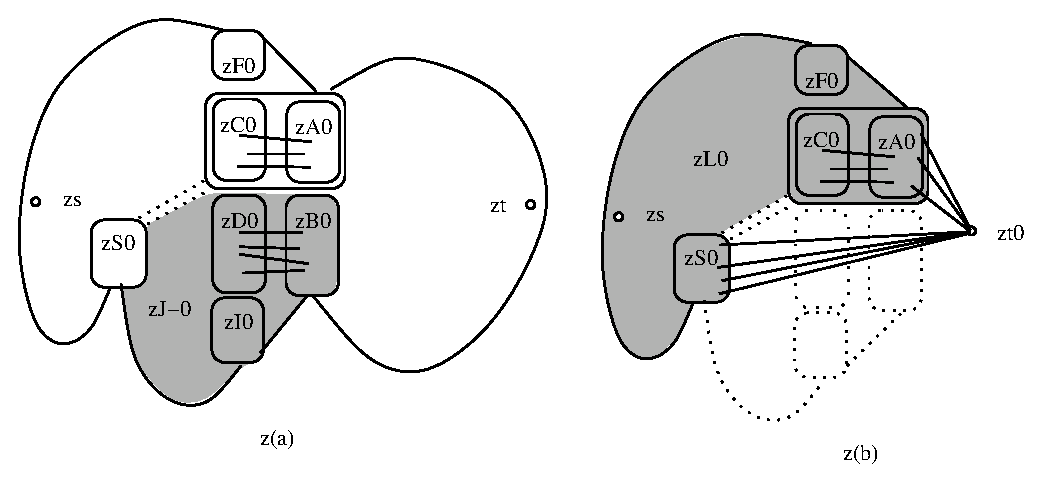
\epsfig{file=fig6.eps, height=5.3cm}
\caption[Fig6]{$J_-^0$ and $L^0$.}
\label{label_fig6}
\end{center}\end{figure}

As $A_0 \cup S_0$ does not separate $s$ from $t$ in $G$, there are some vertices in $C_0$ which are
incident to edges into $J_-^0$.
\begin{itemize}
\item Let $Q_0  := \{q\in C_0 | q$ is adjacent to at least one vertex in $J_-^0$ \}.
\item Let $Q'_0 := \{q'\in V(J_-^0) | q'$ is adjacent to at least one vertex in $Q_0$ \}.
\end{itemize}
From the $s$-$t$ connectivity of $G$, we claim $|Q_0|\ge |B_0|-|S_0|$, and $|Q'_0|\ge |B_0|-|S_0|$.
Please observe that both $S_0\cup Q_0 \cup A_0$ and $S_0\cup Q'_0 \cup A_0$ form $s$-$t$ separators in $G$
(Fig. \ref{label_fig7}(a)).

For the induction process, we consider two graphs $L_R^n$ and $J_R^n$ as follows,
where $n$ indicates a number of iterations.
First, let $J_Q^0$ be a graph based on the subgraph of $G$ induced by $V(J_+^0)\cup Q_0$,
and augmented by two new vertices $u_0$ and $w$, and new edges between $u_0$ and all the vertices in $S_0 \cup Q_0$,
and new edges between all the vertices in $B_0$ and $w$ (Fig. \ref{label_fig7}(b)).
We claim $\kappa_{J_Q^0}(u_0, w) \ge |B_0|$. Suppose not.
Then there would be a minimum $u_0$-$w$ separator $U_0$ such that $|U_0| < |B_0|$.
However, $U_0\cup A_0$ would form an $s$-$t$ separator in $G$, which contradicts the minimality of $X$.
Please note that there is no edge between $L^0 - (S_0\cup A_0)$ and $J_-^0$ except $E(Q_0, Q'_0)$.


\begin{figure}\begin{center}
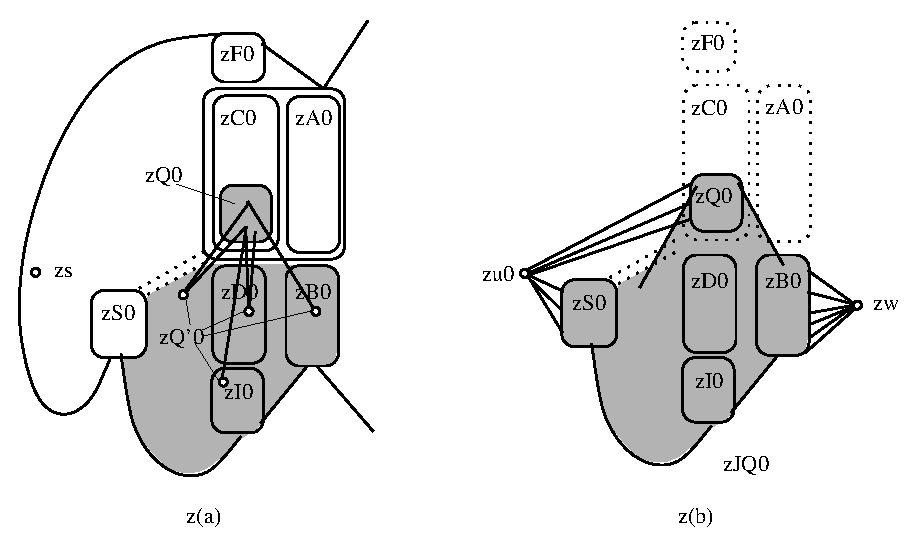
\epsfig{file=fig7.eps, height=7cm}
\caption[Fig7]{$Q_0$, $Q'_0$, and $J_Q^0$.}
\label{label_fig7}
\end{center}\end{figure}

By Proposition \ref{prop1}, we can find at least one subset $R_0$ of $Q_0$ such that $|R_0| = |B_0| - |S_0|$ and
$\kappa_{J_Q^0 - (Q_0\backslash R_0)}(u_0, w) = |B_0|$.
Let the family of such sets be ${\cal R}_0$, and pick any set $R_0$ in ${\cal R}_0$.
Let $J_R^0 := J_Q^0 - (Q_0\backslash R_0)$, and
let $L_R^0$ be a graph based on $L^0$ augmented by new edges between all the vertices in $R_0$ and $t_0$
(Fig. \ref{label_fig8}).
It is easy to see $\kappa_{L_R^0}(s, t_0) \ge |X|$, since existence of an $s$-$t_0$ separator whose cardinality
is less than $|X|$ in $L_R^0$ implies that such a separator would also be an $s$-$t$ separator in $G$.
Also, that $A_0\cup R_0\cup S_0$ form an $s$-$t_0$ separator implies $\kappa_{L_R^0}(s, t_0) = |X|$, and
 $A_0\cup R_0\cup S_0$ form a minimum $s$-$t_0$ separator.

\begin{figure}\begin{center}
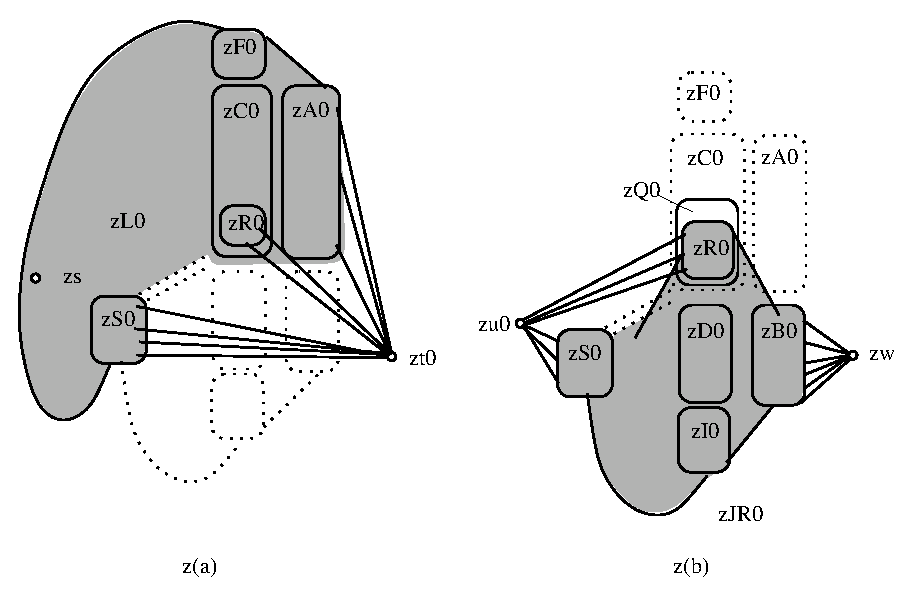
\epsfig{file=fig8.eps, height=7cm}
\caption[Fig8]{$J_R^0$ and $L_R^0$.}
\label{label_fig8}
\end{center}\end{figure}

Let $X_1 := A_0$ and $Y_1 := F_0\cup (C_0\backslash R_0)$.
Let $M_1$ be any bipartite matching of the bipartition $\{Y_1,\,\, X_1\}$.
Existence of the matching is proven using the Hall's marriage theorem similar to the proof of existence of $M_1$.

If $\kappa_{L_R^0/M_1}(s, t_0) \ge |X|$, we set $L_R^n := L_R^0$, $J_R^n := J_R^0$, and we are done.
So we assume $\kappa_{L_R^0/M_1}(s, t_0) < |X|$.

$L_R^0/{M_1}$ has an $s$-$t_0$ separator $W_1$ such that
$|W_1| < |X|$. $W_1$ contains at least one vertex in $V_{M_1}$, otherwise $W_1$ would also be an $s$-$t$ separator
in $G$ whose cardinality is less than $|X|$, a contradiction.
So $W_1\cap V_{M_1}\ne \emptyset$. Let $K_1 = W_1\cap V_{M_1}$ and $S_1 = W_1 \backslash K_1$.

Here we categorize the edges and vertices in $L_R^0$ according to $W_1$
similar to the discussion above when we found $W_0$ (Fig \ref{label_fig9}(a)).
\begin{itemize}
\item Let $E_{K_1}$ be the set of edges in $L_R^0$ which corresponds to $K_1$ in $L_R^0/M_1$.
\item Let $E_{K'_1}$ be $M_1\backslash E_{K_1}$.
\item Let $A_1$ and $C_1$ be the sets of vertices in $X_1$ and $Y_1$ respectively,
which are incident to the edges in $E_{K_1}$.
\item Let $B_1$ and $D_1$ be the sets of vertices in $X_1$ and $Y_1$ respectively,
which are incident to the edges in $E_{K'_1}$.
\item Let $F_1$ be the set of vertices in $Y_1\backslash (C_1\cup D_1)$ which are not incident to any vertices in $B_1$.
\item Let $I_1$ be the set of vertices in $Y_1\backslash (C_1\cup D_1)$ which are incident to any vertices in $B_1$.
\end{itemize}
Please observe that $A_1 \cup C_1 \cup S_1$ separates $s$ from $t_0$ in $L_R^0$,
since $K_1 \cup S_1$ separates $s$ from $t_0$ in $L_R^0/M_1$.
Please also note that $S_1$ can be $\emptyset$, but neither $B_1$ nor $D_1$ can be empty.

\begin{figure}\begin{center}
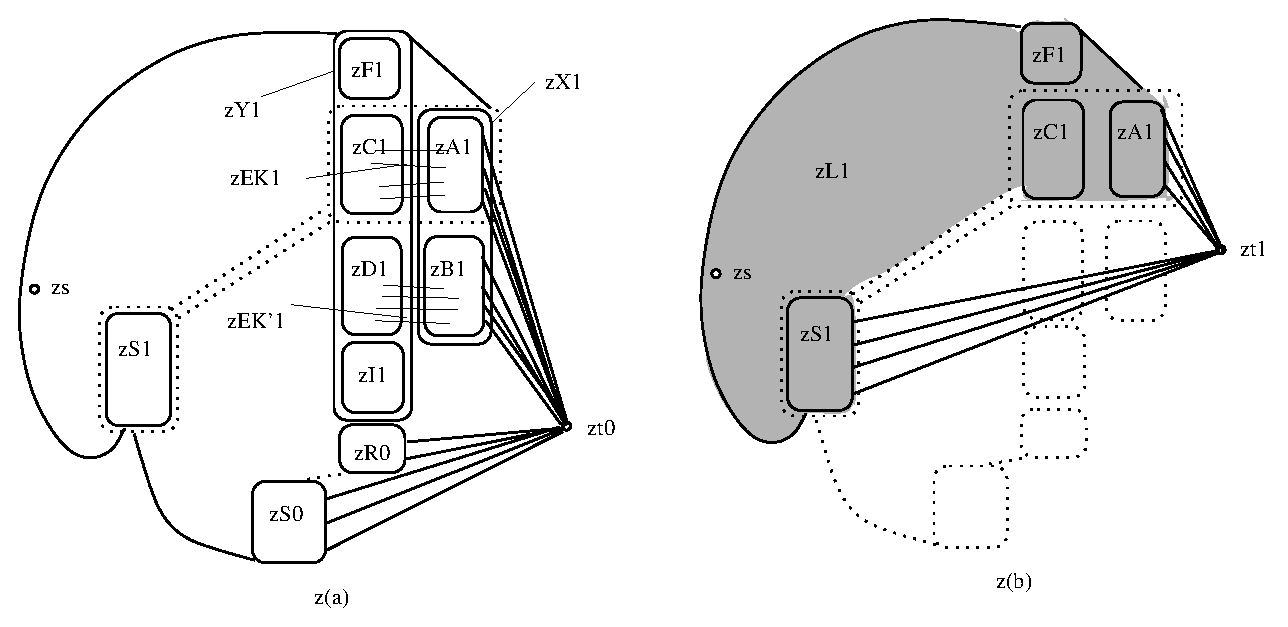
\epsfig{file=fig9.eps, height=5.7cm}
\caption[Fig9]{Subsets of $L_R^0$ and $L^1$.}
\label{label_fig9}
\end{center}\end{figure}

Here we further define two subgraphs of $L_R^0$ and one new graph as follows.
\begin{itemize}
\item Let $J_-^1$ be the component of $L_R^0 - (A_1 \cup C_1 \cup S_1)$ to which $t_0$ belongs.
\item Let $J_+^1$ be a subgraph of $L_R^0$ induced by $V(J_-^1)\cup S_1$.
\item Let $L^1$ be a graph based on $L_R^0 - J_-^1$ augmented by a new vertex $t_1$,
and new edges between $t_1$ and all the vertices in $A_1 \cup S_1$ (Fig \ref{label_fig9}(b)).
\end{itemize}
Also please note that $F_1$ belongs to $L^1$ and $I_1$ belongs to $J_-^1$.

As $A_1 \cup S_1$ does not separate $s$ from $t_0$ in $L_R^0$, there are some vertices in $C_1$ which are
incident to edges into $J_-^1$.
\begin{itemize}
\item Let $Q_1  := \{q\in C_1 | q$ is adjacent to at least one vertex in $J_-^1$ \}.
\item Let $Q'_1 := \{q'\in V(J_-^1) | q'$ is adjacent to at least one vertex in $Q_1$ \}.
\end{itemize}
From the $s$-$t_0$ connectivity of $L_R^0$, we claim $|Q_1|\ge |B_1|+|R_0|+|S_0|-|S_1|$, 
and $|Q'_1|\ge |B_1|+|R_0|+|S_0|-|S_1|$.
Please observe that both $S_1\cup Q_1 \cup A_1$ and $S_1\cup Q'_1 \cup A_1$ form $s$-$t_0$ separators in $L_R^0$.

Let $J_Q^1$ be a graph based on the subgraph of $G$ induced by $V(J_+^1)\cup Q_1$,
and augmented by two new vertices $u_1$ and $w_1$, and new edges between $u_1$ and all the vertices in $S_1 \cup Q_1$,
and new edges between all the vertices in $B_1 \cup R_0 \cup S_0$ and $w_1$.
We claim $\kappa_{J_Q^1}(u_1, w_1) \ge |B_0|+|B_1|$ similar to the reasoning for $\kappa_{J_Q^0}(u_0, w) \ge |B_0|$.
Please note that $|B_1| = |R_0| + |S_0|$.
By Proposition \ref{prop1}, we can find at least one subset $R_1$ of $Q_1$ such that $|R_1| = |B_0|+|B_1| - |S_1|$ and
$\kappa_{J_Q^1 - (Q_1\backslash R_1)}(u_1, w_1) = |B_0|+|B_1|$.
Let the family of such sets be ${\cal R}_1$ and pick any $R_1$ in ${\cal R}_1$.
Let $J_R^1$ be a graph based on $J_R^0 - u_0$ and $J_Q^1 - (Q_1\backslash R_1) - w_1$,
pasted along ${S_0 \cup R_0}$, and add new edges between $B_1$ and $w$ (Fig \ref{label_fig10}(a)).
Please note that $J_R^1 - \{u_1, w\}$ is an induced subgraph of $G$.

\begin{figure}\begin{center}
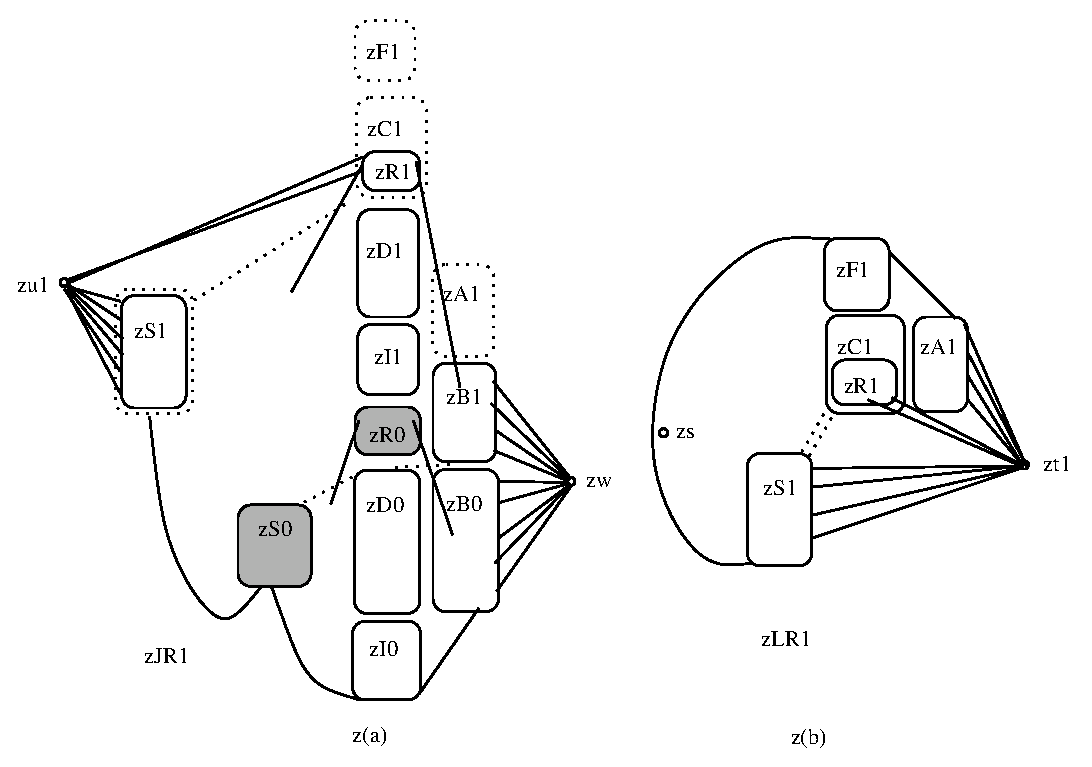
\epsfig{file=fig10.eps, height=8cm}
\caption[Fig10]{Subsets of $J_R^1$ and $L_R^1$.}
\label{label_fig10}
\end{center}\end{figure}

Let $L_R^1$ be a graph based on $L^1$ augmented by new edges between all the vertices in $R_1$ and $t_1$
(Fig \ref{label_fig10}(b)).
It is easy to see $\kappa_{L_R^1}(s, t_1) = |X|$
due to the similar reasoning for $\kappa_{L_R^0}(s, t_0) = |X|$,
and $A_1\cup R_1\cup S_1$ form a minimum $s$-$t_1$ separator in $L_R^1$.

We repeat this process $n$ times until we obtain $L_R^n$, $J_R^n$,
such that there is a bipartite matching $M_n$ for $L_R^n$ such that $\kappa_{L_R^n/M_n}(s, t_n) = |X|$
(Fig \ref{label_fig11}).

\begin{figure}\begin{center}
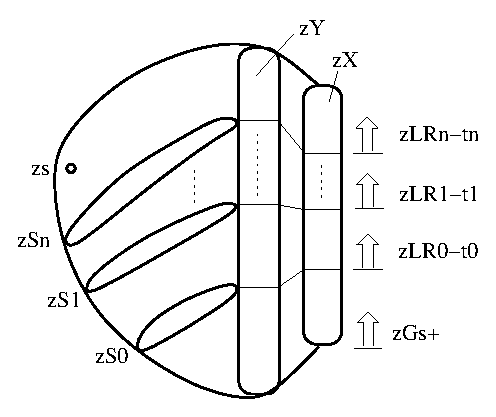
\epsfig{file=fig11.eps}
\caption[Fig11]{$G_s^+, L_R^0, \ldots, L_R^n$.}
\label{label_fig11}
\end{center}\end{figure}

This process is guaranteed to terminate at the $n$-th iteration due to the following reason.
Assume we are at the $i$-th iteration. Let $\alpha_i = \kappa_{L_R^i}(s, t_i) - \kappa_{L_R^i/M_i}(s, t_i)$.
The discussion above implies the necessary condition for $\alpha_i$ to be any positive integer
is existence of $R_i$ in $F_i \cup C_i$ such that $|R_i| = \alpha_i$, and $|A_i| \le |F_i \cup (C_i \backslash R_i)|$.
Thus, taking the contraposition, $\alpha_i$ has to be less than or equal to $|Y_i| - |X_i|$.
However, $|Y_{i-1}| - |X_{i-1}| > |Y_{i}| - |X_{i}|$ due to existence of $R_{i-1}$.
This implies that $\alpha_i$ is strictly monotone decreasing,
and there exists $n \in {\bf N}$ such that at the $n$-th iteration,
$\alpha_n = 0$.

Also, $V(L_R^n)\cap |X| \ne \emptyset$.
So $V(J_R^n)\cap |X|$ is a proper subset of $X$, and $\kappa_{J_R^n}(u_n, w) < |X|$.
By the induction hypothesis, $J_R^n$ has a bipartite matching $M'_n$ of $V(J_R^n)\cap |X|$
such that $\kappa_{J_R^n/M'_n}(u_n, w) = \kappa_{J_R^n}(u_n, w)$.
Finally we obtain a bipartite matching $M_n \cup M'_n$ of $X$ in $G_s^+$, contraction of which does not decrease the
$s$-$t$ connectivity of $G$. {\bf Q.E.D.}



\bibliography{menger}
\end{document}



